%%%%%%%%%%%%%%%%%%%%%%%%%%%%%%%%%%%%%%%%%%%%%%%%%%%%%%%%
%%%%                                              %%%%%%
%%%%  Author: Peter Wilson                        %%%%%%
%%%%                                              %%%%%%
%%%%  Composite shells                        %%%%%%
%%%%                                              %%%%%%
%%%%%%%%%%%%%%%%%%%%%%%%%%%%%%%%%%%%%%%%%%%%%%%%%%%%%%%%


%fref generates automatically the respective abreviation/word in the text for the reference. You just have to define a label starting with the respective keyword.
%english: chap, sec, fig, eq, app
%deutsch: chap/kap, abs, abb, gl, anh
%see http://ctan.space-pro.be/tex-archive/macros/latex/contrib/fancyref/fancyref.pdf for more \section

%\onehalfspacing
%\setlength{\belowcaptionskip}{-17pt}

\chapter{Composite shells - revised 1}
\label{chap:chapter_2_1}

\renewcommand{\Thema}{Composite shells}

\lettrine[lines=2]{A}{s} is the case with shell structures, anisotropic structures are widely encountered throughout the natural and man-made environment. Truly isotropic materials are but a subset of naturally occurring structures, with the phenotypical material often being anisotropic due to varying environmental pressure in different directions. Intuitively, inspecting the ongoing genetic optimization of constructions forming the natural environment suggests that the best mechanical behaviour for a structure subject to spatially non-uniform requirements will be non-uniform itself. This same philosophy has recently began to dominate the cutting edge of man-made engineering structures where specialized high-performance is demanded, leading to greater adoption of composite materials. The increasing proportion of composite materials in the aerospace industry is but one example of their increasing traction.

\begin{figure}[H]
	\centering
	\def\svgwidth{\columnwidth}
	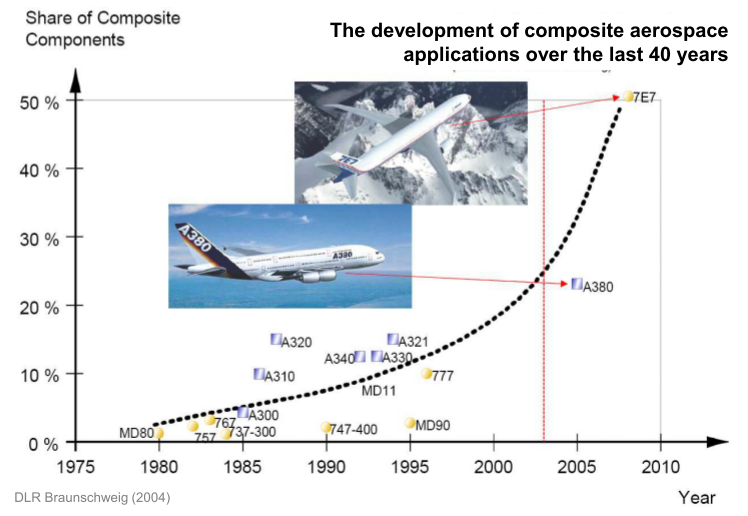
\includegraphics[width=14cm]{images/composites_aerospace.png}
	\caption{Material composition of the Boeing 787 \cite{AMCA2017}}
	\label{composite_aerospace}
\end{figure}

The reason behind this increased propensity to use composites in high performance engineering applications is their customisability. Material properties such conductivity, density, wear resistance, and directional stiffness can be tailored to suit the exact needs of a design region. Directionally-varying stiffness is effectively leveraged in modern carbon-fiber road bicycles by simultaneously providing high stiffness for efficient power transfer and deliberate compliance for rider comfort and increased traction. This is one example of a composite material fulfilling seemingly mutually exclusive objectives due to finely tuned material properties built upon a knowledge of composite material basics.

\section{Composite material basics}

Composite materials are typically the combination of a high strength/stiffness fibre reinforcement material and a weaker/softer base matrix material. Although a wide range composites exist, they are broadly grouped into fibrous composites (employing fibre reinforcement materials), particulate composites (employing particle reinforcement materials) and laminate composites composed of layers of different materials, including fibrous and particulate composites. Of these, this work focusses on laminates composed of fibrous composites which are commonly used in practical engineering.

\subsection{Laminae and laminates}

Laminae are individual layers or plies of composite materials, which, when stacked together, form a laminate. Each lamina consists of a volume percentage of reinforcement fibres embedded within a matrix material, aligned at a particular orientation to some coordinate system. Common fibre reinforcement materials are various glass fibres (including E-glass and S-glass), carbon/graphite fibres and boron fibres while common matrix materials are thermosetting polymers such as polyester and epoxy resins and metals including aluminium and titanium. The reinforcement fibres may be arranged in the lamina matrix in a variety of patterns and orientations, either continuous or discontinuous \cite{agarwal2006analysis}. 
\begin{figure}[H]
	\subfloat[Various composite laminae]
	{\label{ref_label2}
		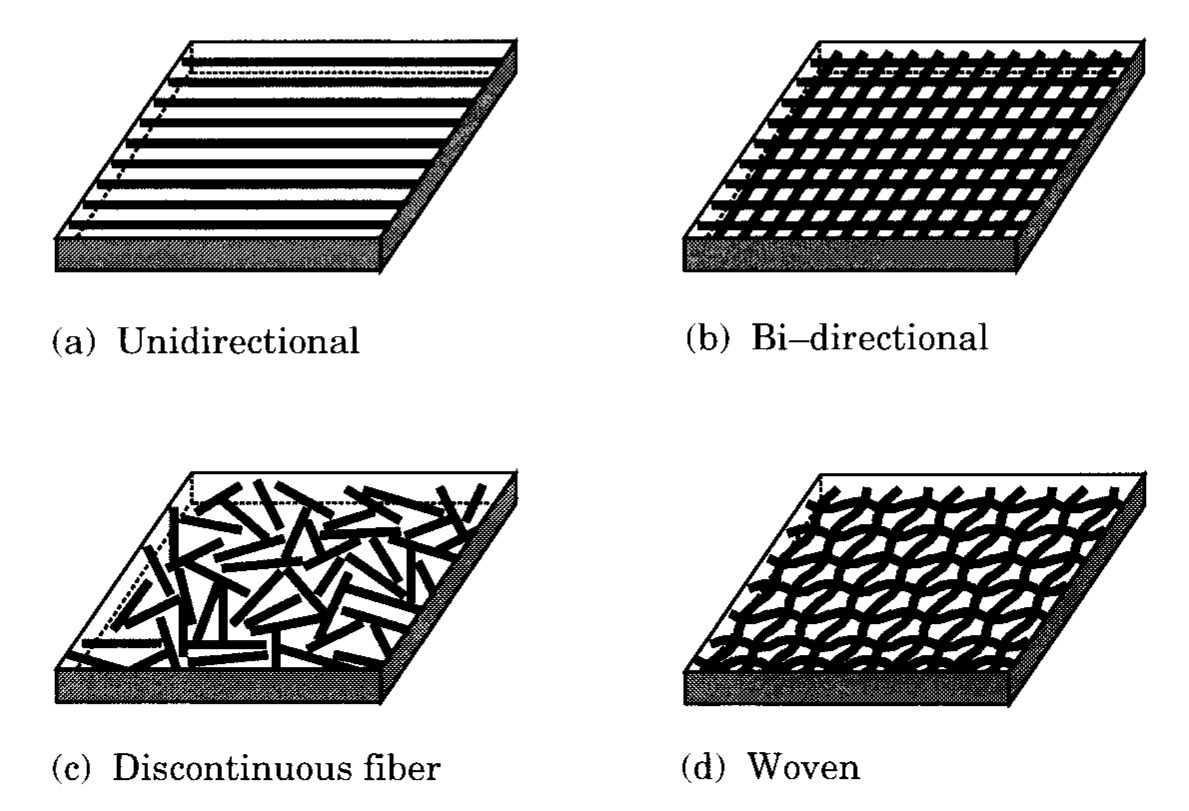
\includegraphics[width=7.3cm]
		{images/composite_laminae.png}}
	\subfloat[Composite laminate composed of laminae arranged in a stacking sequence]
	{\label{ref_label2}
		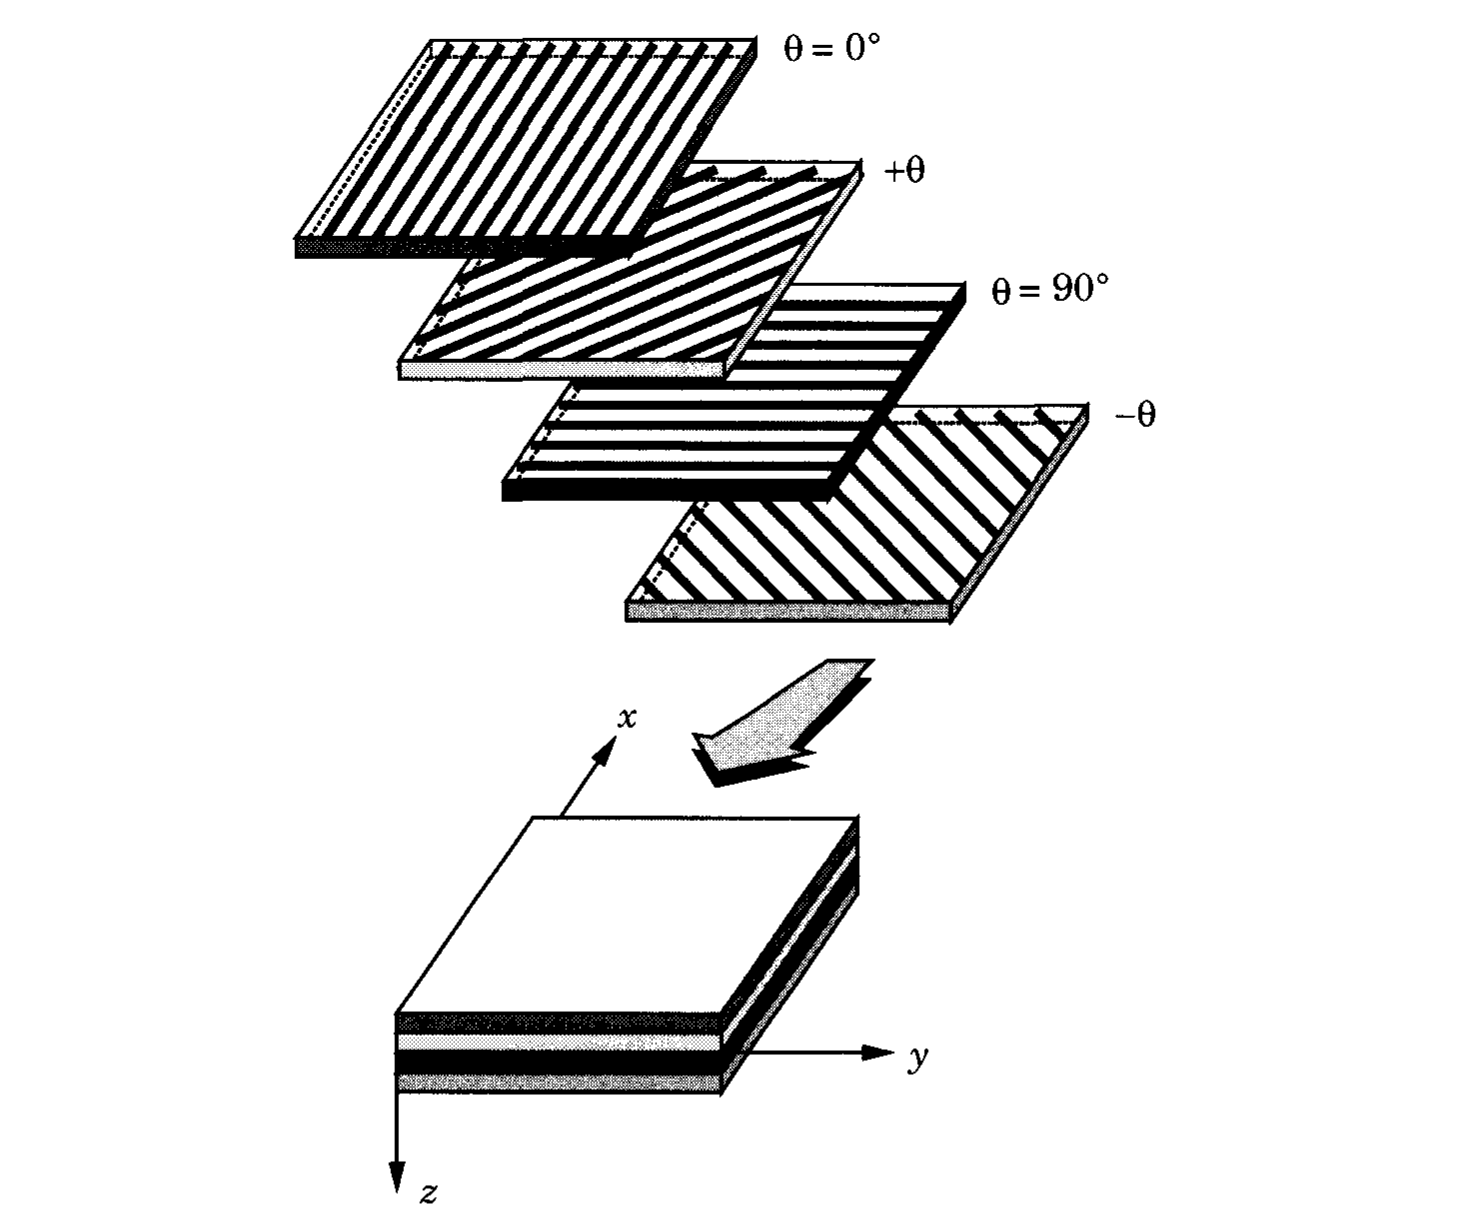
\includegraphics[width=7.3cm]
		{images/composite_laminates.png}}
	\caption{\label{composite_laminates}Components of composite laminates \cite{reddy2004mechanics}}
\end{figure}

Considering the four laminae in figure \ref{composite_laminates}(a) examples of anisotropy to varying degrees can be intuited. The unidirectional continuous fibre pattern is incredibly stiff and strong in the fibre direction while being relatively compliant and weak  perpendicular to this fibre direction. Contrasting this, a practically in-plane isotropic lamina may be achieved with very fine discontinuous fibres randomly oriented within the matrix substrate. Thus, the importance of individual lamina makeup forms a critical determinant of the structural behaviour of the total laminate as a whole. Another critical determinant of the laminate behaviour is the stacking sequence of the laminate, which prescribes the number of laminae, their vertical order and their orientation as per figure \ref{composite_laminates}(b). The control that these two determinants offer designers facilitate highly optimized structures for well defined structural requirements.

An industrial example of this is spoolable Glass Reinforced Epoxy (GRE) oil piping, which has a central GRE structural lamina sandwiched between two non-structural Polyethylene (PE) laminae intended to provide the structural layer chemical and environmental protection. Furthermore, the fibre alignment of the GRE structural lamina is often orientated at an optimal pressure-capacity angle since the stress field of the pipe operating under internal pressure is well defined.

\subsection{Constitutive equations of orthotropic laminae}

A pre-requisite of modelling complex laminates is the characterisation of each lamina. The general constitutive equations of laminae are thus established under the assumption of perfectly continuous linear elastic materials without fibre breakages or matrix voids. For a generally anisotropic material the stresses can be related to the strains as follows:

\begin{equation} 
\sigma^{ij} = C_0^{ijkl} \epsilon_{kl}
\label{eqscomp1}
\end{equation}

Equivalently, adopting Reddy's \cite{reddy2004mechanics} notation:

\begin{equation} 
\begin{pmatrix}
\sigma_{11} \\
\sigma_{22} \\
\sigma_{33} \\
\sigma_{23} \\
\sigma_{13} \\
\sigma_{12}
\end{pmatrix}
=
\begin{pmatrix}
C_{11} & C_{12} & C_{13} & C_{14} & C_{15} & C_{16} \\
\  & C_{22} & C_{23} & C_{24} & C_{25} & C_{26} \\
\  & \  & C_{33} & C_{34} & C_{35} & C_{36} \\
\  & \  & \  & C_{44} & C_{45} & C_{46} \\
\  & sym. & \  & \ & C_{55} & C_{56} \\
\  & \  & \  & \  & \  & C_{66}
\end{pmatrix}
\begin{pmatrix}
\epsilon_{11} \\
\epsilon_{22} \\
\epsilon_{33} \\
2\epsilon_{23} \\
2\epsilon_{13} \\
2\epsilon_{12}
\end{pmatrix}
\label{eqscomp2}
\end{equation}

The preceding discussion of laminae illustrated there are innumerable design variants for any lamina. In practise however, one of the most common lamina arrangements are orthotropic laminae. Orthotropic laminae have three mutually orthogonal planes of symmetry, which reduces the unique entries of the lamina-orientated constitutive tensor from 21 (anisotropic materials) to 9:

\begin{equation} 
\begin{pmatrix}
\sigma_{11} \\
\sigma_{22} \\
\sigma_{33} \\
\sigma_{23} \\
\sigma_{13} \\
\sigma_{12}
\end{pmatrix}
=
\begin{pmatrix}
C_{11} & C_{12} & C_{13} & 0 & 0 & 0 \\
\  & C_{22} & C_{23} & 0 & 0 & 0 \\
\  & \  & C_{33} & 0 & 0 & 0 \\
\  & \  & \  & C_{44} & 0 & 0 \\
\  & sym. & \  & \ & C_{55} & 0 \\
\  & \  & \  & \  & \  & C_{66}
\end{pmatrix}
\begin{pmatrix}
\epsilon_{11} \\
\epsilon_{22} \\
\epsilon_{33} \\
2\epsilon_{23} \\
2\epsilon_{13} \\
2\epsilon_{12}
\end{pmatrix}
\label{eqscomp3}
\end{equation}

Furthermore, if the lamina is suitably thin, as is typically the case in composite shell structures, a state of plane stress can be assumed. This corresponds to $\sigma_{33} = 0$ as per the following illustration.

\begin{figure}[h!]
	\centering
	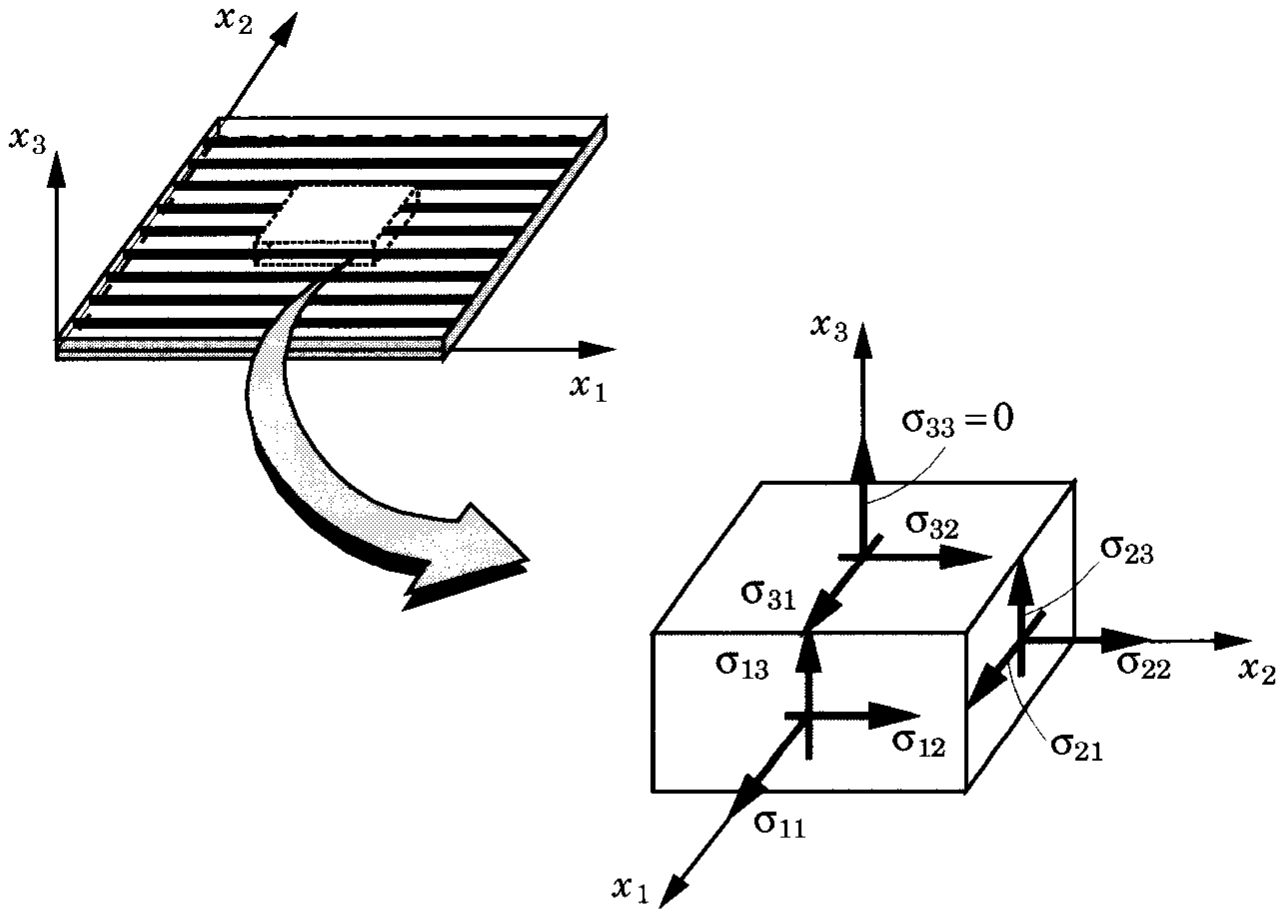
\includegraphics[width=12cm]{images/composite_lamina_plane_stress}
	\caption{Lamina in a plane stress state \cite{reddy2004mechanics}}
	\label{fig:compositelaminaplanestress}
\end{figure}


The reduced plane stress orthotropic lamina constitutive tensor is therefore:

\begin{equation} 
\begin{pmatrix}
\sigma_{11} \\
\sigma_{22} \\
\sigma_{12} \\
\sigma_{23} \\
\sigma_{13} 
\end{pmatrix}
=
\begin{pmatrix}
Q_{11} & Q_{12} &  0 & 0 & 0 \\
\  & Q_{22} &  0 & 0 & 0 \\
\  & \  & Q_{66}  & 0 & 0 \\
\  & sym. & \  & Q_{44} & 0 \\
\  & \  & \  & \ & Q_{55}
\end{pmatrix}
\begin{pmatrix}
\epsilon_{11} \\
\epsilon_{22} \\
2\epsilon_{12}\\
2\epsilon_{23} \\
2\epsilon_{13}
\end{pmatrix}
\label{eqscomp_plane_stress_tensor_unrotated}
\end{equation}

The entries $Q_{ij}$ are derived from the bulk structural properties of the lamina at the macro-mechanical level. For example, the bulk lamina properties of a continuous fibre unidirectional design depicted in the following figure is considered.

\begin{figure}[H]
	\centering
	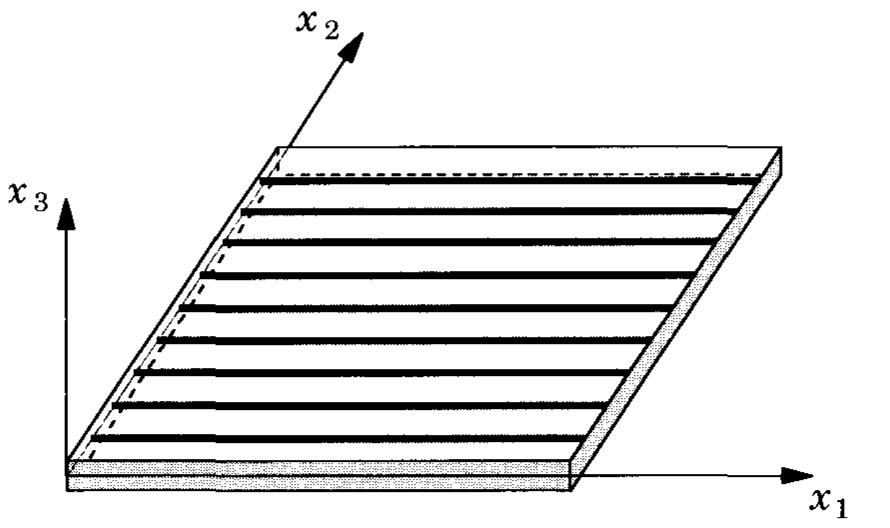
\includegraphics[width=10cm]{images/composite_unidirectional_lamina}
	\caption{Continuous unidirectional fibre lamina arrangement \cite{reddy2004mechanics}}
	\label{fig:compositeunidirectionallamina}
\end{figure}

If the Young's moduli and the Poisson ratios of both the individual fibre ($E_f,\ \nu_f$) and matrix ($E_m,\ \nu_m$) materials are known, along with the volume fraction of each ($v_f,\ v_m$), the resulting bulk lamina moduli can be determined. 

Consider that the bulk modulus $E_1$, along $x_1$ and parallel to the fibres, is activated by tension $\sigma_{11}$ along $x_1$. The constraint $\epsilon_{11_f} = \epsilon_{11_m} = \epsilon_{11}$ must be satisfied at every cross sectional area $A$ along $x_1$. Thus:
\begin{equation} 
\sigma_{11} = E_1\epsilon_{11}\ ,
\hspace{10mm}
\sigma_{11_f} = E_f\epsilon_{11_f}\ ,
\hspace{10mm}
\sigma_{11_m} = E_m\epsilon_{11_m}
\label{eqscomp5}
\end{equation}
Applying force equilibrium:
\begin{equation} 
\sigma_{11}A = \sigma_{11_f}A v_f + \sigma_{11_m}A v_m
\label{eqscomp6}
\end{equation}
Substituting and rearranging yields the bulk longitudinal Young's modulus of the lamina:
\begin{equation} 
E_1 = E_f v_f + E_m v_m
\label{eqscomp7}
\end{equation}
A similar line of analysis can be performed for the other lamina moduli, yielding the following results:
\begin{equation} 
E_2 = \frac{E_f E_m}{E_f v_m + E_m v_f}\ ,
\hspace{10mm}
\nu_{12} = \nu_f v_f + \nu_m v_m\ ,
\hspace{10mm}
G_{12} = \frac{G_f G_m}{G_f v_m + G_m v_f}
\label{eqscomp8}
\end{equation}

The example of continuous unidirectional fibre laminae highlight that the material description of laminae can be shifted from a micro-mechanical level to a macro-mechanical level characterised by equivalent parameters. These are related to the entries $Q_{ij}$ of the reduced plane stress orthotropic lamina constitutive tensor in equation \ref{eqscomp_plane_stress_tensor_unrotated} as follows:

\begin{equation} 
Q_{11} = \frac{E_1}{1-\nu_{12} \nu_{21}}\ ,
\hspace{10mm}
Q_{12} = \frac{\nu_{12} E_1}{1-\nu_{12} \nu_{21}}\ ,
\hspace{10mm}
Q_{22} = \frac{E_2}{1-\nu_{12} \nu_{21}}
\label{eqscomp9}
\end{equation}
\begin{equation} 
Q_{66} = G_{12}\ ,
\hspace{10mm}
Q_{44} = G_{23}\ ,
\hspace{10mm}
Q_{55} = G_{13}
\label{eqscomp10}
\end{equation}

The lamina macro-mechanical parameters $E_1,\ E_2,\ \nu_{12}, G_{12},\ G_{23}$ and $G_{13}$ can be derived from the micro-mechanical properties of the lamina, as demonstrated, or, as is more common, are obtained experimentally. Regardless of their method of origin, these parameters are always aligned with the lamina local coordinate system, which may not necessarily coincide with the laminate coordinate system, or, more generally, the global reference coordinate system of the analysis.

\begin{figure}[h!]
	\centering
	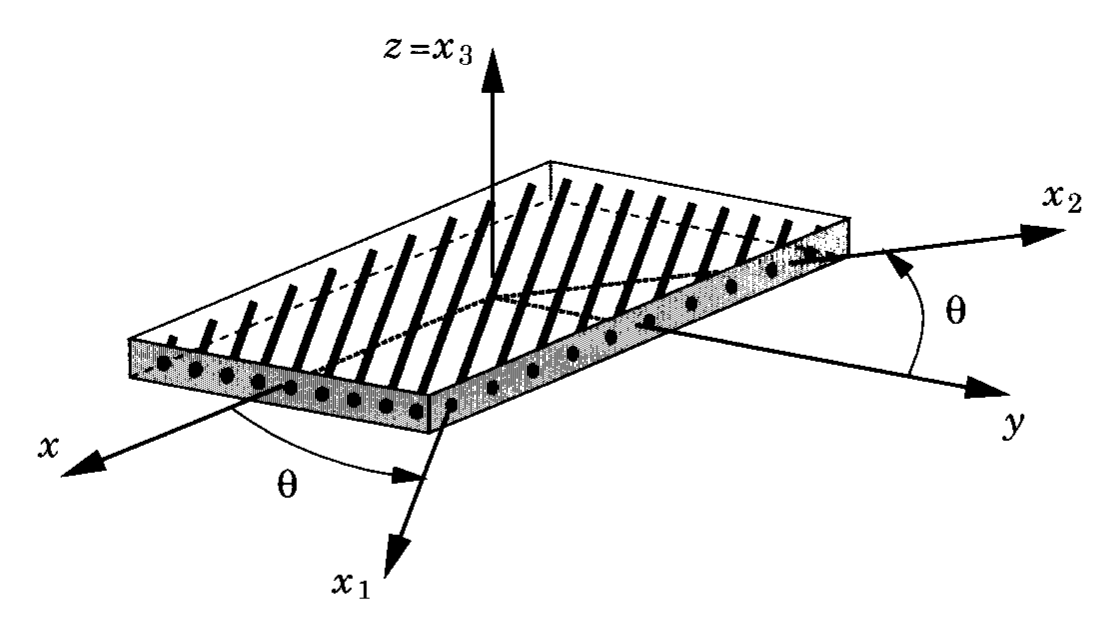
\includegraphics[width=12cm]{images/composite_lamina_orientation}
	\caption{Arbitrary orientation of lamina \cite{reddy2004mechanics}}
	\label{fig:compositelaminaorientation}
\end{figure}

The transformation of a locally oriented ($x_1,\ x_2,\ x_3$) lamina constitutive tensor $\mathbf{Q}$ to one aligned with a reference coordinate system ($x,\ y,\ z$) $\bar{\mathbf{Q}}$ through an angle $\theta$ about $\mathbf{z}=\mathbf{x_3}$ is achieved as follows ($c = cos\theta,\ s = sin\theta$):
\begin{equation} 
\bar{\mathbf{Q}} = \mathbf{T}^T \mathbf{Q} \mathbf{T}\ ,
\hspace{10mm}
\mathbf{T} =
\begin{pmatrix}
c^2 & s^2 & -2sc & 0 & 0 \\
s^2 & c^2 & 2sc & 0 & 0 \\
sc & -sc & c^2 - s^2 & 0 & 0 \\
0 & 0 & 0 & c & s \\
 0 & 0 & 0 & -s & c
\end{pmatrix}
\label{eqscomp11}
\end{equation}
Thus, stresses and strains in the reference coordinate system  ($x,\ y,\ z$) are related as such:
\begin{equation} 
\begin{pmatrix}
\sigma_{xx} \\
\sigma_{yy} \\
\sigma_{xy} \\
\sigma_{yz} \\
\sigma_{xz} 
\end{pmatrix}
=
\begin{pmatrix}
\bar{Q}_{11} & \bar{Q}_{12} &  \bar{Q}_{16} & 0 & 0 \\
\  & \bar{Q}_{22} &  \bar{Q}_{26} & 0 & 0 \\
\  & \  & \bar{Q}_{66}  & 0 & 0 \\
\  & sym. & \  & \bar{Q}_{44} & \bar{Q}_{45} \\
\  & \  & \  & \ & \bar{Q}_{55}
\end{pmatrix}
\begin{pmatrix}
\epsilon_{xx} \\
\epsilon_{yy} \\
2\epsilon_{xy}\\
2\epsilon_{yz} \\
2\epsilon_{xz}
\end{pmatrix}
\label{eqscomp_plane_stress_tensor_rotated}
\end{equation}

This transformation is required to correctly assemble laminae in laminates that have non-zero stacking angles, which, by virtue of their customizability, is almost all laminates. With the individual lamina constitutive behaviour detailed, orthotropic shell laminates can now be built up and modelled.

\section{Orthotropic shell laminates: internal virtual work}

Orthotropic shell laminates are composites made from a stacking sequence of orthotropic laminae. As per their application in shells, the assumption of plane stress is continued.

The 5 parameter shell theory internal virtual work is recalled as:
\begin{equation} 
-\delta\Pi_{int} =
\int_\Omega
\boldsymbol{\epsilon}
:
\mathbf{C}_{mem}
:
\delta \boldsymbol{\epsilon}\ d \Omega\ 
+
\int_\Omega
\boldsymbol{\kappa}
:
\mathbf{C}_{bend}
:
\delta \boldsymbol{\kappa}\ 
d \Omega\ 
+
\int_\Omega
\boldsymbol{\gamma}
:
\mathbf{C}_{shear}
:
\delta \boldsymbol{\gamma}\ 
d \Omega
\label{eqsrm4_in_composite1}
\end{equation}

The integral over the volume can split into area and laminate thickness integrals:
\begin{equation} 
-\delta\Pi_{int} =
\int_h
\int_A
\boldsymbol{\sigma}_{mem}
:
\delta \boldsymbol{\epsilon}\ dAdh\ 
+
\int_h
\int_A
\boldsymbol{\sigma}_{bend}
:
\delta \boldsymbol{\kappa}\ 
\ dAdh\ 
+\\
\int_h
\int_A
\boldsymbol{\tau}
:
\delta \boldsymbol{\gamma}\ 
\ dAdh
\label{eqsrm4_in_composite2}
\end{equation}

By pre-integrating the stress quantities, and restricting the scope of the equations to 2D plane stress conditions, the following equivalent form can be presented in vector notation:

\begin{equation} 
-\delta\Pi_{int} =
\int_A
\mathbf{N}^T
\delta \boldsymbol{\epsilon}
\ dA\ 
+
\int_A
\mathbf{M}^T
\delta \boldsymbol{\kappa}\ 
\ dA\ 
+
\int_A
\mathbf{Q}^T
\delta \boldsymbol{\gamma}\ 
\ dA
\label{eqsrm4_in_composite3}
\end{equation}

The introduced quantities $\mathbf{N,\ M}$ and $\mathbf{Q}$ are force and moment resultants over the entire laminate as per the following figure:

\begin{figure}[H]
	\centering
	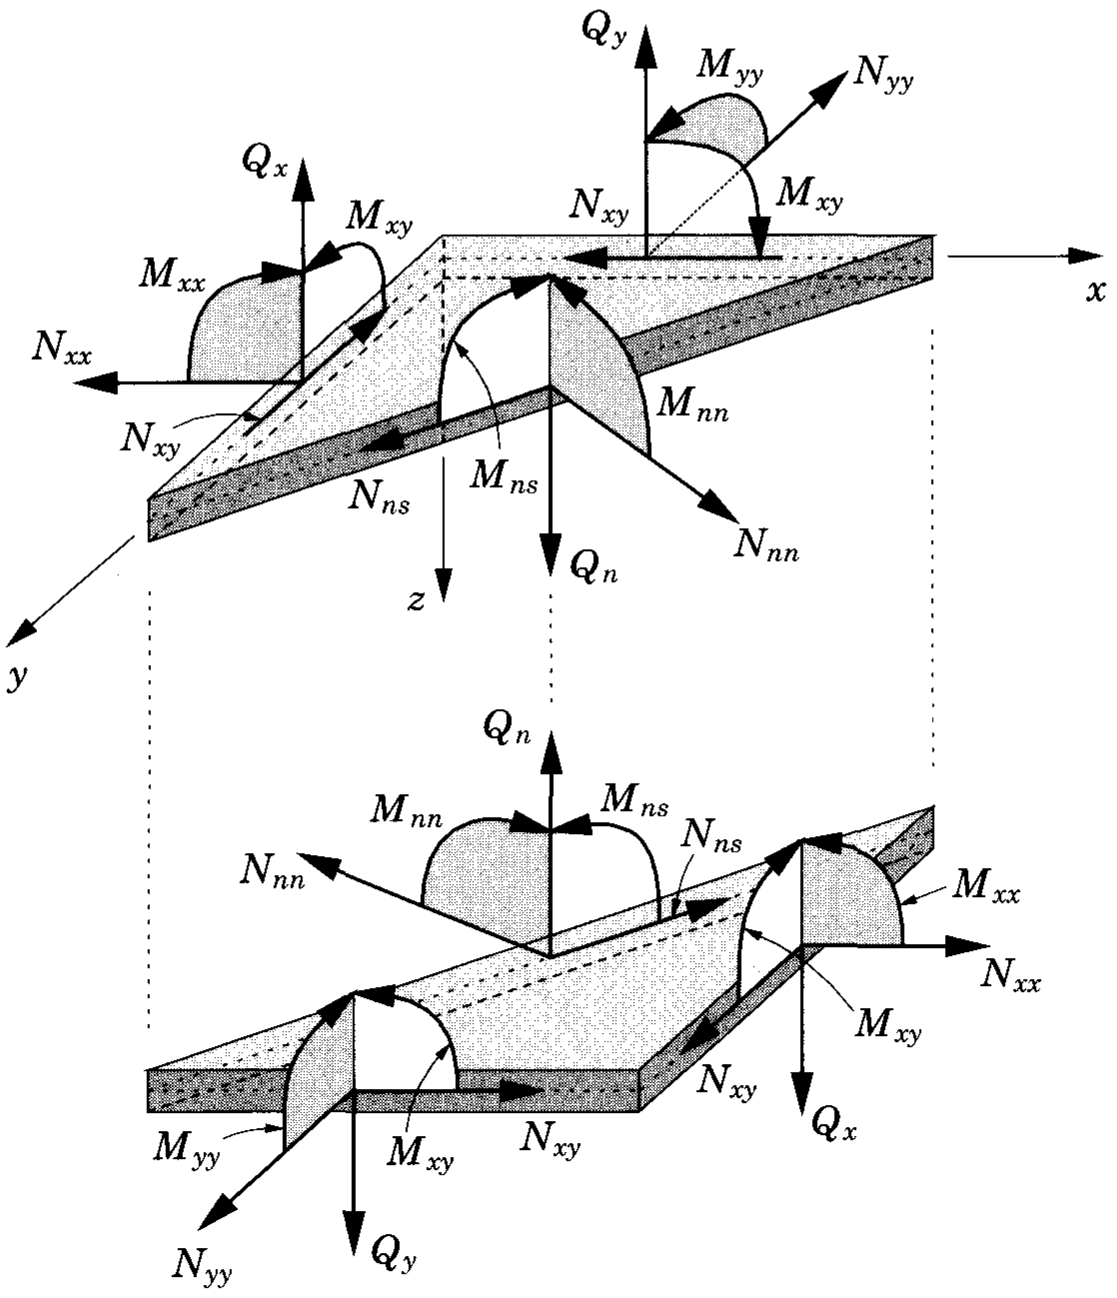
\includegraphics[width=10cm]{images/composite_force_resultants}
	\caption{Force and moment resultants of a plate \cite{reddy2004mechanics}}
	\label{fig:compositeforceresultants}
\end{figure}

The force and moment resultants are defined as follows:

\begin{equation} 
\mathbf{N} = 
\begin{pmatrix}
N_{xx} \\
N_{yy} \\
N_{xy} 
\end{pmatrix}
=
{\int_{\frac{-h}{2}}^{\frac{h}{2}}
\begin{pmatrix}
\sigma_{xx} \\
\sigma_{yy} \\
\sigma_{xy} 
\end{pmatrix}}
dz\ ,
\hspace{5mm}
\mathbf{M} = 
\begin{pmatrix}
M_{xx} \\
M_{yy} \\
M_{xy} 
\end{pmatrix}
=
{\int_{\frac{-h}{2}}^{\frac{h}{2}}
	\begin{pmatrix}
	\sigma_{xx} \\
	\sigma_{yy} \\
	\sigma_{xy} 
	\end{pmatrix}}z\ 
dz
\label{eqscomp_force_resultants}
\end{equation}

The shear resultants only applicable for the 5 parameter model are similarly defined, including a shear energy correction factor of $\alpha = \frac{5}{6}$:

\begin{equation} 
\mathbf{Q} = 
\begin{pmatrix}
Q_{x} \\
Q_{y} 
\end{pmatrix}
= \alpha
{\int_{\frac{-h}{2}}^{\frac{h}{2}}
	\begin{pmatrix}
	\sigma_{xz} \\
	\sigma_{yz} 
	\end{pmatrix}}
dz
\label{eqscomp_force_resultants2}
\end{equation}

\subsection{Laminate constitutive equations}

At this point, the laminate force resultants, by way of the stress integrals, must be related back to strains across all laminae via laminate constitutive equations. A laminate of total thickness $h$ with $n$ laminae is considered below:

\begin{figure}[h!]
	\centering
	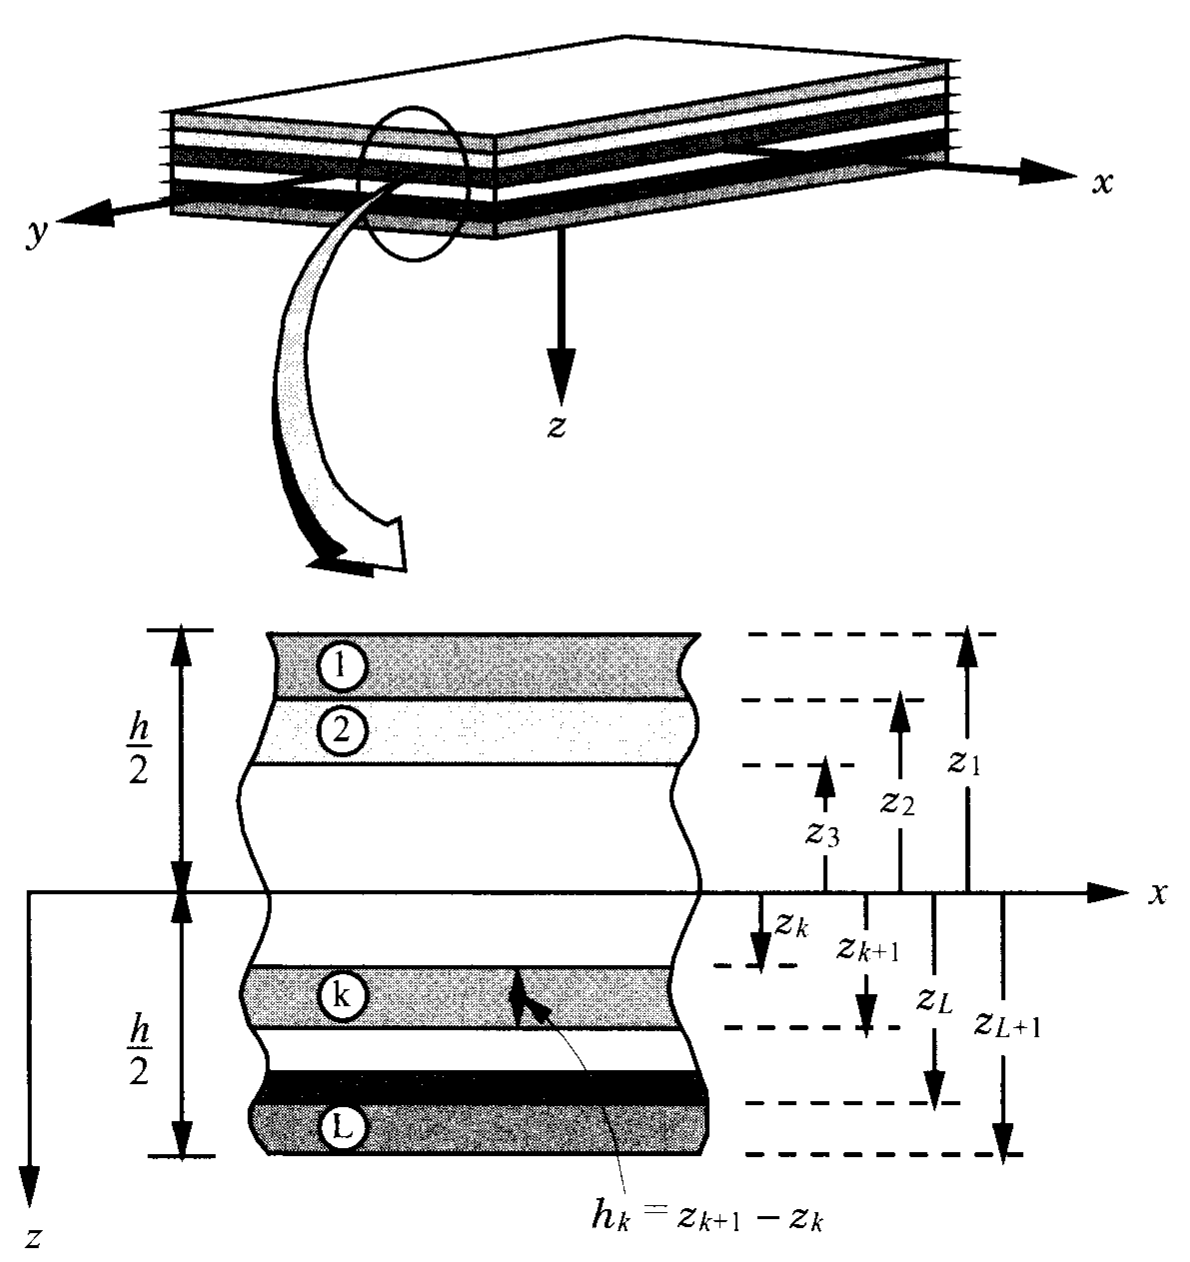
\includegraphics[width=10cm]{images/composite_layer_system}
	\caption{Coordinate system and lamina numbering in a laminate \cite{reddy2004mechanics}}
	\label{fig:compositelayersystem}
\end{figure}

The force resultants can be determined as:

\begin{equation}
\mathbf{N} = 
\begin{pmatrix}
N_{xx} \\
N_{yy} \\
N_{xy} 
\end{pmatrix}
=
{\int_{\frac{-h}{2}}^{\frac{h}{2}}
	\begin{pmatrix}
	\sigma_{xx} \\
	\sigma_{yy} \\
	\sigma_{xy} 
	\end{pmatrix}}
dz
=
\sum_{k=1}^n
\int_{z_k}^{z_{k+1}}
	\begin{pmatrix}
	\sigma_{xx} \\
	\sigma_{yy} \\
	\sigma_{xy} 
	\end{pmatrix}
dz
\label{eqscomp_laminate_constitutive1}
\end{equation}

Invoking the laminae constitutive properties previously established in equation \ref{eqscomp_plane_stress_tensor_rotated} leads to the 'mathematical assemblage' of the laminae into the laminate via the following integral:
\begin{gather} 
	\begin{aligned}
		\begin{pmatrix}
			N_{xx} \\
			N_{yy} \\
			N_{xy} 
		\end{pmatrix} 
		& = 
		\sum_{k=1}^n
		\int_{z_k}^{z_{k+1}}
		{\begin{pmatrix}
			\bar{Q}_{11} & \bar{Q}_{12} &  \bar{Q}_{16} \\
			\bar{Q}_{12} & \bar{Q}_{22} &  \bar{Q}_{26} \\
			\bar{Q}_{16} & \bar{Q}_{26} & \bar{Q}_{66} 
		\end{pmatrix}}^{(k)}
		\begin{pmatrix}
			\epsilon_{xx} + z \kappa_{xx}\\
			\epsilon_{yy} + z \kappa_{xx}\\
			2\epsilon_{xy} + 2z\kappa_{xy}
		\end{pmatrix}
		dz \\
		& =
		\begin{pmatrix}
			{A}_{11} & {A}_{12} &  {A}_{16} \\
			{A}_{12} & {A}_{22} &  {A}_{26} \\
			{A}_{16} & {A}_{26} & {A}_{66} 
		\end{pmatrix}
		\begin{pmatrix}
		\epsilon_{xx}\\
		\epsilon_{yy}\\
		2\epsilon_{xy}
		\end{pmatrix}
		+
		\begin{pmatrix}
		{B}_{11} & {B}_{12} &  {B}_{16} \\
		{B}_{12} & {B}_{22} &  {B}_{26} \\
		{B}_{16} & {B}_{26} & {B}_{66} 
		\end{pmatrix}
		\begin{pmatrix}
		 \kappa_{xx}\\
		\kappa_{xx}\\
		2\kappa_{xy}
		\end{pmatrix}
		\label{eqscomp_laminate_constitutive3}
	\end{aligned}
\end{gather}
Similarly, the moment and shear force resultants can be related to strains:
\begin{gather} 
	\begin{aligned}
		\begin{pmatrix}
			M_{xx} \\
			M_{yy} \\
			M_{xy} 
		\end{pmatrix} 
		& = 
		\sum_{k=1}^n
		\int_{z_k}^{z_{k+1}}
		{\begin{pmatrix}
				\bar{Q}_{11} & \bar{Q}_{12} &  \bar{Q}_{16} \\
				\bar{Q}_{12} & \bar{Q}_{22} &  \bar{Q}_{26} \\
				\bar{Q}_{16} & \bar{Q}_{26} & \bar{Q}_{66} 
		\end{pmatrix}}^{(k)}
		\begin{pmatrix}
			\epsilon_{xx} + z \kappa_{xx}\\
			\epsilon_{yy} + z \kappa_{xx}\\
			2\epsilon_{xy} + 2z\kappa_{xy}
		\end{pmatrix}
		z\ dz \\
		& =
		\begin{pmatrix}
			{B}_{11} & {B}_{12} &  {B}_{16} \\
			{B}_{12} & {B}_{22} &  {B}_{26} \\
			{B}_{16} & {B}_{26} & {B}_{66} 
		\end{pmatrix}
		\begin{pmatrix}
			\epsilon_{xx}\\
			\epsilon_{yy}\\
			2\epsilon_{xy}
		\end{pmatrix}
		+
		\begin{pmatrix}
			{D}_{11} & {D}_{12} &  {D}_{16} \\
			{D}_{12} & {D}_{22} &  {D}_{26} \\
			{D}_{16} & {D}_{26} & {D}_{66} 
		\end{pmatrix}
		\begin{pmatrix}
			\kappa_{xx}\\
			\kappa_{yy}\\
			2\kappa_{xy}
		\end{pmatrix}
		\label{eqscomp_laminate_constitutive4}
	\end{aligned}
\end{gather}
\begin{equation} 
			\begin{pmatrix}
			Q_{x} \\
			Q_{y} 
			\end{pmatrix}
		= \alpha
		\sum_{k=1}^n
		\int_{z_k}^{z_{k+1}}
			{\begin{pmatrix}
			\bar{Q}_{44} & \bar{Q}_{45} \\
			\bar{Q}_{45} & \bar{Q}_{55} 
			\end{pmatrix}}^{(k)}
			\begin{pmatrix}
			2\epsilon_{yz} \\
			2\epsilon_{xz} 
			\end{pmatrix}
		dz
		= \alpha
			{\begin{pmatrix}
			{A}_{44} & {A}_{45} \\
			{A}_{45} & {A}_{55} 
			\end{pmatrix}}
			\begin{pmatrix}
			2\epsilon_{yz} \\
			2\epsilon_{xz} 
			\end{pmatrix}
		\label{eqscomp_laminate_constitutive5}
\end{equation}

The three introduced matrices represent the extensional stiffnesses $A_{ij}$, the bending stiffnesses $D_{ij}$ and the bending-extensional coupling stiffnesses $B_{ij}$, and are determined from the lamina stiffnesses $\bar{Q}_{ij}^{(k)}$:

\begin{equation} 
	A_{ij} = 
	\int_{\frac{-h}{2}}^{\frac{h}{2}}
	\bar{Q}_{ij}
	\ dz\ ,
	\hspace{5mm}
	B_{ij} = 
	\int_{\frac{-h}{2}}^{\frac{h}{2}}
	\bar{Q}_{ij}\ z
	\ dz\ ,
	\hspace{5mm}
	D_{ij} = 
	\int_{\frac{-h}{2}}^{\frac{h}{2}}
	\bar{Q}_{ij}\ z^2
	\ dz
	\label{eqscomp_laminate_constitutive6}
\end{equation}

By organising the resultants into a generalised resultant vector $\bar{\mathbf{N}}$ and the strains into a generalized strain vector $\bar{\boldsymbol{\epsilon}}$, the following summary is produced:

\begin{equation} 
\bar{\mathbf{N}} = \bar{\mathbf{C}} \bar{\boldsymbol{\epsilon}} =
\begin{pmatrix}
N_{xx} \\
N_{yy} \\
N_{xy} \\
M_{xx} \\
M_{yy} \\
M_{xy} \\
Q_{x} \\
Q_{y} 
\end{pmatrix} 
=
\begin{pmatrix}
\mathbf{A} & \mathbf{B} & \mathbf{0} \\
\mathbf{B} & \mathbf{D} & \mathbf{0} \\
\mathbf{0}& \mathbf{0} & \alpha		\begin{pmatrix}
								{A}_{44} & {A}_{45} \\
 								{A}_{45} & {A}_{55} 
 								\end{pmatrix} 
\end{pmatrix} 
\begin{pmatrix}
\epsilon_{xx} \\
\epsilon_{yy} \\
2\epsilon_{xy}\\
\kappa_{xx}\\
\kappa_{yy}\\
2\kappa_{xy} \\
2\epsilon_{yz} \\
2\epsilon_{xz}
\end{pmatrix}
\label{eqscomp_laminate_constitutive7}
\end{equation}

The internal virtual work of the 5 parameter shell model presented in equation \ref{eqsrm4_in_composite3} can therefore be reduced down to: 

\begin{equation} 
-\delta\Pi_{int} =
\int_A
\bar{\mathbf{N}}^T
\delta \bar{\boldsymbol{\epsilon}}
\ dA
\label{eqscomp_laminate_constitutive8}
\end{equation}

\section{Laminate strain and stress recovery}
\label{Laminate strain and stress recovery}

Critical to the practical design of laminates is the evaluation of stresses and strains not only on the laminate mid-plane, but throughout the thickness across laminae. The following describes the procedure of recovering these quantities at arbitrary positions within the laminate thickness.

\subsection{Laminate strain recovery}

Owing to the dimensional reduction from 3D to 2D, the generalized shell strains $\bar{\boldsymbol{\epsilon}}$ of equation \ref{eqscomp_laminate_constitutive7} are referred to the mid-plane $(z=0)$ of the laminate. Thus, within a local convective laminate coordinate system describing the z-axis orientation as per figure \ref{fig:compositelayersystem}:

\begin{equation} 
\bar{\boldsymbol{\epsilon}} (x,\ y) = \boldsymbol{\epsilon} (x,\ y,\ 0)
\label{eqscomp_strain_recovery1}
\end{equation}

A consequence of the straight director assumption common to both the 3 and 5 parameter shell models is the membrane strains vary proportionally to the distance from the mid-plane. This can be observed in the following diagram of a plate in pure bending highlighting the linear variation of in-plane stresses (which, in simple cases, are merely scaled strains):

\begin{figure}[H]
	\centering
	\def\svgwidth{\columnwidth}
	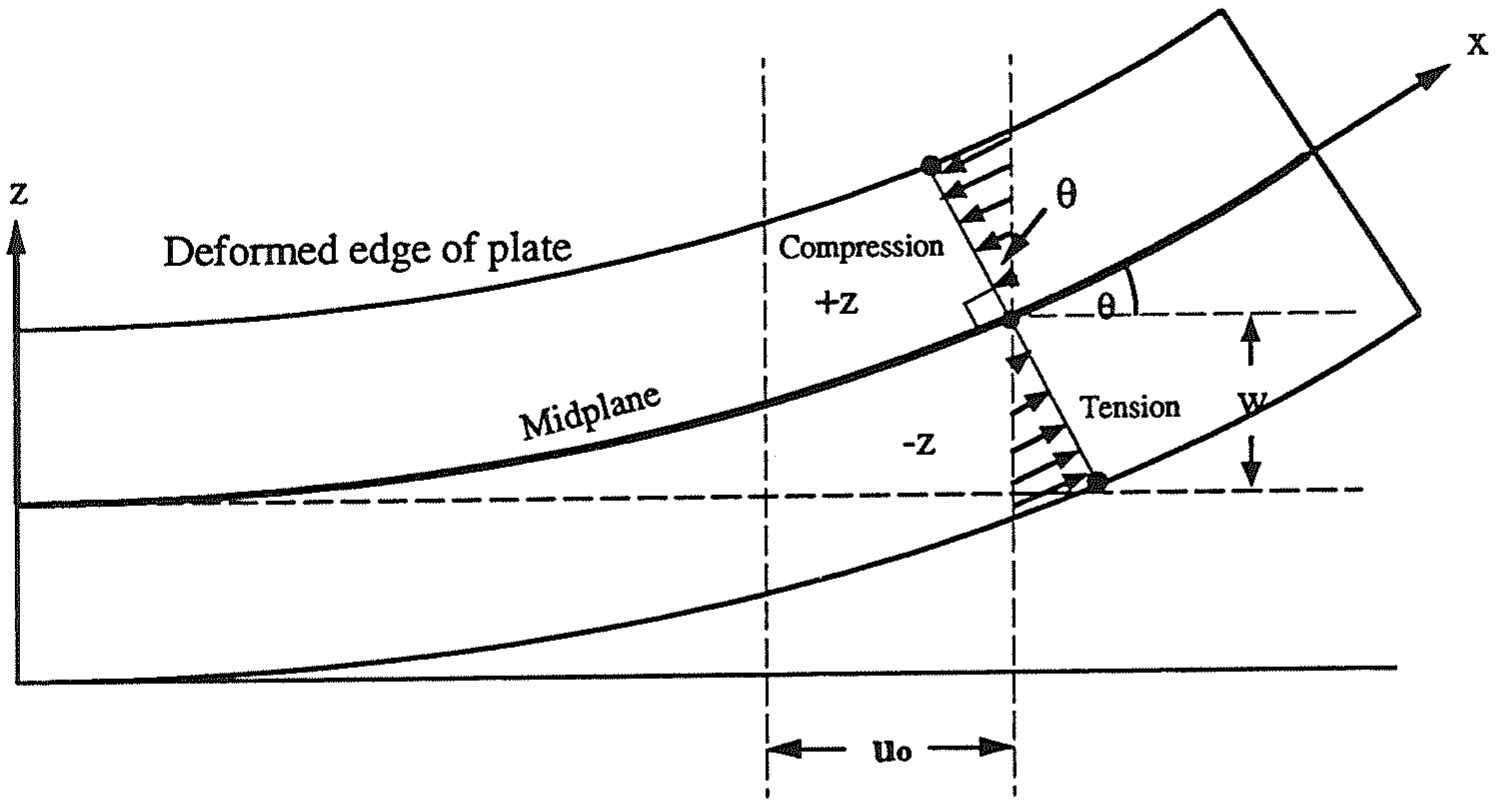
\includegraphics[width=12cm]{images/composite_nasa_strains.png}
	\caption{Deformation of 3 parameter plate \cite{nasanettles1994}}
	\label{fig:compositenasastrains}
\end{figure}

Thus the in-plane strains at any position $z$ in the laminate are determined from:
\begin{equation} 
\begin{pmatrix}
\epsilon_{xx} \\
\epsilon_{yy} \\
2\epsilon_{xy}\\
\end{pmatrix}_{(z)}
=
\begin{pmatrix}
\epsilon_{xx} \\
\epsilon_{yy} \\
2\epsilon_{xy}\\
\end{pmatrix}_{(z=0)}
+
z
\begin{pmatrix}
\kappa_{xx}\\
\kappa_{yy}\\
2\kappa_{xy} \\
\end{pmatrix}_{(z=0)}
\label{eqscomp_strain_recovery2}
\end{equation}

The in-plane strains of a surface in any lamina within the laminate can be determined by appropriately setting the corresponding $z$ value.

Applicable only to 5 parameter shell models is the recovery of transverse shear strains. A perusal of Kreja's literature review on composite models \cite{kreja2011literature} indicates the amount of academic effort dedicated to accurately modelling transverse shear strains in first order shear deformation theories. The contradiction driving this effort is that 5 parameter models are limited to expressing constant transverse shear strain over the shell thickness, while it is known that for an isotropic material they are actually distributed parabolically. This is the reason behind the shear correction factor of $\alpha = \frac{5}{6}$ which is actually the ratio of internal transverse shear strain energy in a 5 parameter plate to that of 3D elasticity. Without delving into exotic laminate shell theories, two options for recovering the transverse shear strain avail themselves: (1) accept the limitations of the 5 parameter model and consider the transverse shear strain constant across the section, or; (2) reconstruct a parabolic profile from the mid-plane values, as is often done for isotropic materials.

The first approach of accepting constant transverse shear stress is expressed as follows:

\begin{equation} 
\begin{pmatrix}
2\epsilon_{yz} \\
2\epsilon_{xz}
\end{pmatrix}_{(z)}
=
\begin{pmatrix}
2\epsilon_{yz} \\
2\epsilon_{xz}
\end{pmatrix}_{(z=0)}
\label{eqscomp_strain_recovery3}
\end{equation}

The second approach of constructing a parabolic strain profile using limiting expressions from \cite{FelippaKirchhoff2017} is described below, starting with the distribution of the transverse shear stress $\sigma_{xz}$ in an isotropic plate:
\begin{equation} 
\sigma_{xz} (z) = \sigma_{xz}^{max} (1-\frac{4z^2}{h^2})  = \frac{3Q_x}{2h} (1-\frac{4z^2}{h^2}) = \frac{3}{2} \sigma_{xz}^{av} (1-\frac{4z^2}{h^2})
\label{eqscomp_strain_recovery4}
\end{equation}

Unlike laminate stresses, which are generally discontinuous across the thicknesss, laminate strains are continuous. Therefore, the strain distribution of the isotropic plate will be transferred to the laminate.
The strain distribution of an isotropic plate must follow the stress distribution, thus:
\begin{equation} 
\gamma_{xz} (z)=  \frac{3}{2} \gamma_{xz}^{av} (1-\frac{4z^2}{h^2}) = \frac{3}{2} 2\epsilon_{xz}^{(z=0)} (1-\frac{4z^2}{h^2})
\label{eqscomp_strain_recovery5}
\end{equation}

Summarising, the approximated transverse shear distribution for the laminate is:
\begin{equation} 
\begin{pmatrix}
2\epsilon_{yz} \\
2\epsilon_{xz}
\end{pmatrix}_{(z)}
=
\frac{3}{2} (1-\frac{4z^2}{h^2})
\begin{pmatrix}
2\epsilon_{yz} \\
2\epsilon_{xz}
\end{pmatrix}_{(z=0)}
\label{eqscomp_strain_recovery6}
\end{equation}

The in-plane and transverse shear strains determined thus far are referred to the reference coordinate system of the laminate $(x,\ y,\ z)$. However, it is often of interest to transform these strains so they are aligned with the individual lamina considered $(x_1,\ y_1,\ z_1)$. For a lamina oriented at $\theta$ to the laminate coordinate system, the strain components can be transformed as such ($c = cos\theta,\ s = sin\theta$):

\begin{equation} 
\begin{pmatrix}
\epsilon_{11} \\
\epsilon_{22} \\
2\epsilon_{12}\\
2\epsilon_{23} \\
2\epsilon_{13}
\end{pmatrix}
 =
\begin{pmatrix}
c^2 & s^2 & sc & 0 & 0 \\
s^2 & c^2 & -sc & 0 & 0 \\
-sin2\theta & sin2\theta & c^2 - s^2 & 0 & 0 \\
0 & 0 & 0 & c & -s \\
0 & 0 & 0 & s & c
\end{pmatrix}
\begin{pmatrix}
\epsilon_{xx} \\
\epsilon_{yy} \\
2\epsilon_{xy}\\
2\epsilon_{yz} \\
2\epsilon_{xz}
\end{pmatrix}
\label{eqscomp_strain_recovery7}
\end{equation}

\subsection{Laminate stress recovery}

With the laminate strains across the thickness described, the stresses can be recovered by simply applying the considered lamina constitutive law as per equation \ref{eqscomp_plane_stress_tensor_rotated}. Naturally, the material coefficients $Q_{ij}$ should correspond to the $k^{th}$ lamina considered at the height of inspection $z$:

\begin{equation} 
{\begin{pmatrix}
\sigma_{xx} \\
\sigma_{yy} \\
\sigma_{xy} \\
\sigma_{yz} \\
\sigma_{xz} 
\end{pmatrix}}_{(z)}
=
{\begin{pmatrix}
\bar{Q}_{11} & \bar{Q}_{12} &  \bar{Q}_{16} & 0 & 0 \\
\  & \bar{Q}_{22} &  \bar{Q}_{26} & 0 & 0 \\
\  & \  & \bar{Q}_{66}  & 0 & 0 \\
\  & sym. & \  & \bar{Q}_{44} & \bar{Q}_{45} \\
\  & \  & \  & \ & \bar{Q}_{55}
\end{pmatrix}}_{(k)}
{\begin{pmatrix}
\epsilon_{xx} \\
\epsilon_{yy} \\
2\epsilon_{xy}\\
2\epsilon_{yz} \\
2\epsilon_{xz}
\end{pmatrix}}_{(z)}
\label{eqscomp_stress_recovery1}
\end{equation}

As previously implied, although the strain distribution is continuous across laminates, the stress distribution is generally discontinuous due to the varying material properties of the laminae. Indeed, if the laminae of a laminate are the exact same orthotropic composite material, but are stacked at varying angles, the resulting stress distribution will be discontinuous. The following example of a 4 ply laminate with a [0, 45, 45, 0] stacking sequence subject to pure bending highlights the nature of stress and strain distributions through the thickness despite all laminae being the same material.

\begin{figure}[H]
	\subfloat[Continuous strain distribution]
	{\label{ref_label2}
		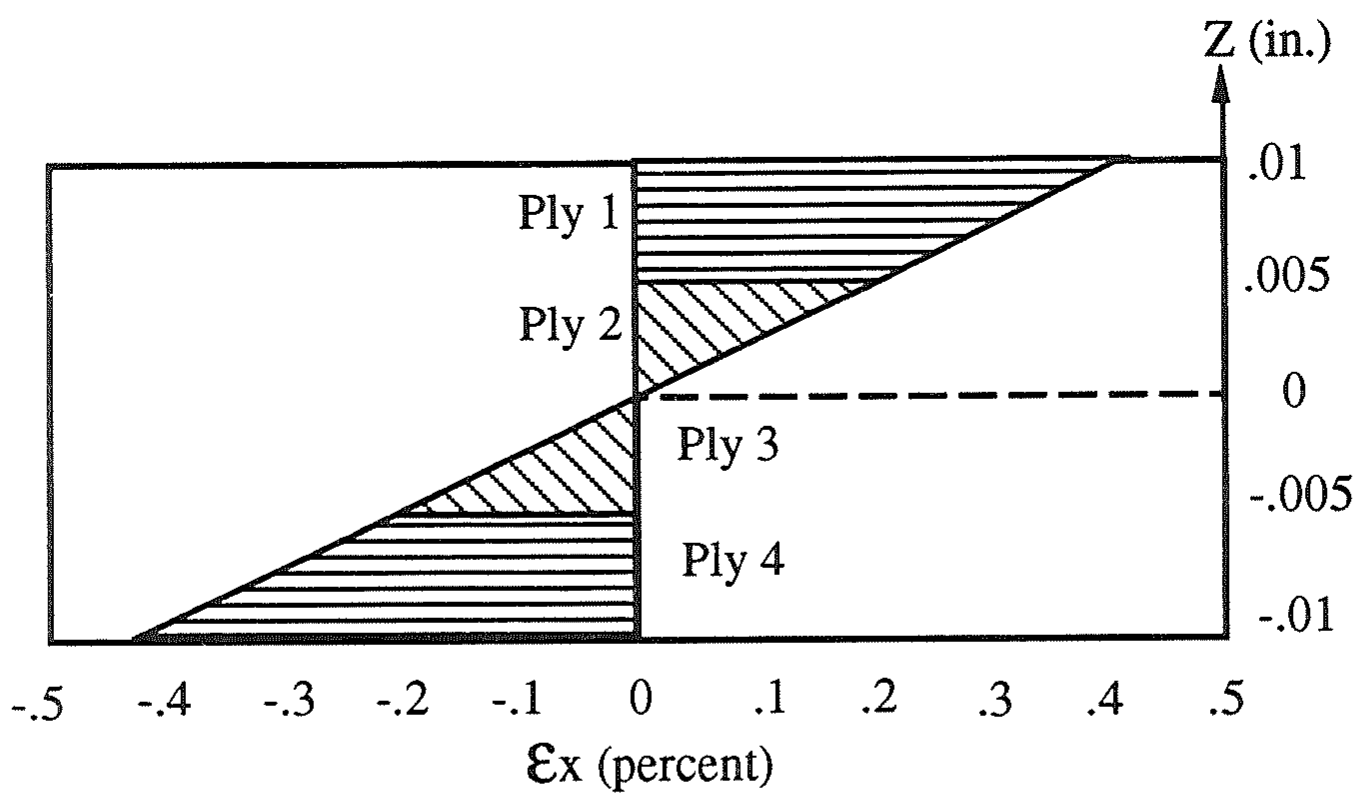
\includegraphics[width=7.3cm]
		{images/composite_nasa_strain_ex1.png}}
	\subfloat[Discontinuous stress distribution]
	{\label{ref_label2}
		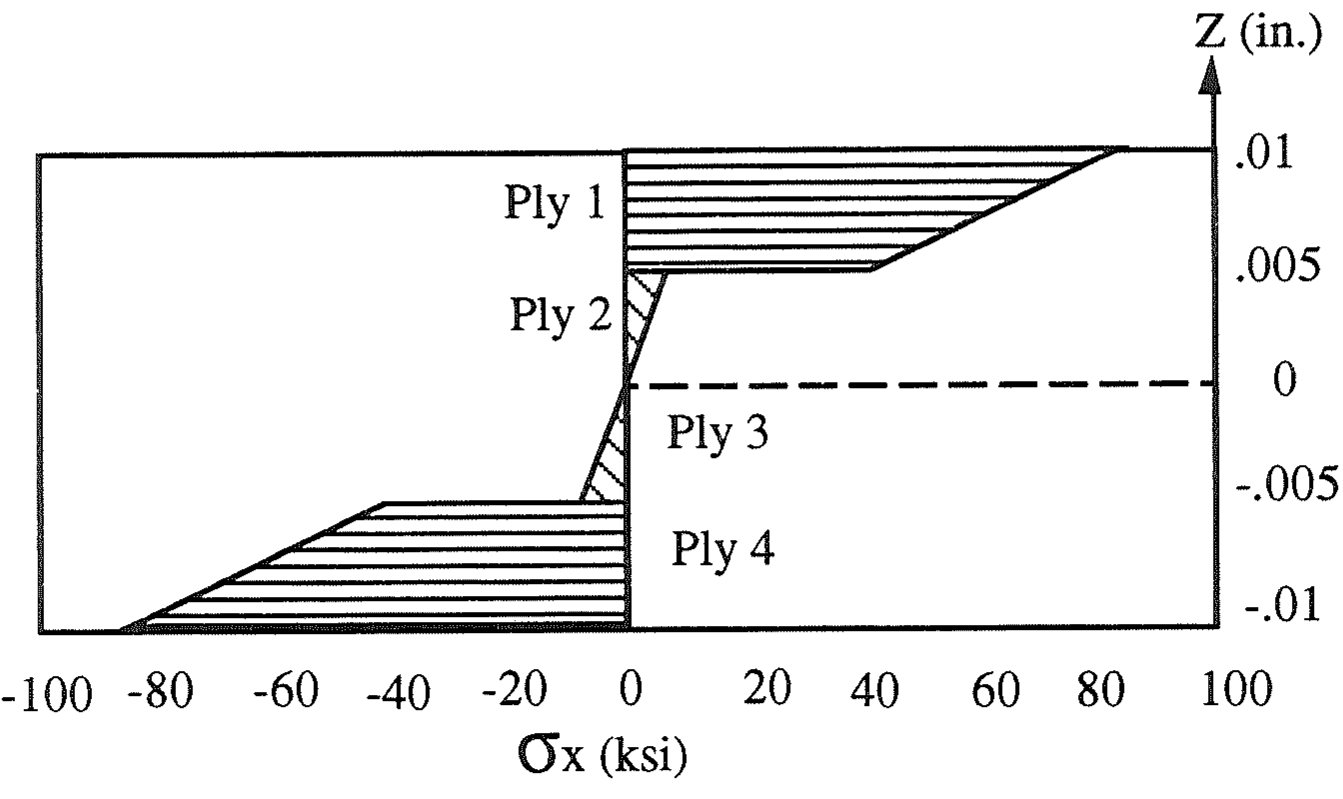
\includegraphics[width=7.3cm]
		{images/composite_nasa_stress_ex1.png}}
	\caption{\label{composite_stress_strain}Stress and strain thickness distribution of 4 ply plate subject to pure bending  \cite{nasanettles1994}}
\end{figure}

Similar to the laminate strains, the in-plane and transverse shear stresses determined thus far are referred to the reference coordinate system of the laminate. For a lamina oriented at $\theta$ to the laminate coordinate system $(x,\ y,\ z)$, the stress components can be transformed to the lamina coordinate system $(x_1,\ y_1,\ z_1)$ as such ($c = cos\theta,\ s = sin\theta$):

\begin{equation} 
\begin{pmatrix}
\sigma_{11} \\
\sigma_{22} \\
2\sigma_{12}\\
2\sigma_{23} \\
2\sigma_{13}
\end{pmatrix}
=
\begin{pmatrix}
c^2 & s^2 & sin2\theta & 0 & 0 \\
s^2 & c^2 & -sin2\theta & 0 & 0 \\
-sc & sc & c^2 - s^2 & 0 & 0 \\
0 & 0 & 0 & c & -s \\
0 & 0 & 0 & s & c
\end{pmatrix}
\begin{pmatrix}
\sigma_{xx} \\
\sigma_{yy} \\
2\sigma_{xy}\\
2\sigma_{yz} \\
2\sigma_{xz}
\end{pmatrix}
\label{eqscomp_stress_recovery2}
\end{equation}

\section{Laminate Tsai-Wu failure criterion}
\label{tsai wu background}
The Tsai-Wu failure criterion is a relatively simple method to approximate the safety of composite materials under combined loading. As an extension of the Von Mises distortion energy theory, it provides an invariant scalar indication of how proximate the current stress state of a lamina is to breaching the closed convex failure surface \cite{tsai12}. The closed convex failure surface is defined by material strength parameters $F_i$ and $F_{ij}$, with failure predicted by fulfilling the following inequality \cite{reddy2004mechanics}:

\begin{equation} 
\sum_{i=1}^{6} F_i \sigma_i + \sum_{i=1}^{6} \sum_{j=1}^{6} F_{ij} \sigma_{ij} \geq 1.0
\hspace{10mm}with\hspace{10mm}
\begin{pmatrix}
\sigma_{1} \\
\sigma_{2} \\
\sigma_{3}\\
\sigma_{4} \\
\sigma_{5} \\
\sigma_{6}
\end{pmatrix}
=
\begin{pmatrix}
\sigma_{11} \\
\sigma_{22} \\
\sigma_{33}\\
\sigma_{23} \\
\sigma_{13} \\
\sigma_{12}
\end{pmatrix}
\label{eqscomp_tsai1}
\end{equation}

By considering the tensile $(X_T,\ Y_T,\ Z_T)$ and compressive $(X_C,\ Y_C,\ Z_C)$ strengths in the lamina principal material directions (1, 2, 3) and the shear strengths $(R,\ S,\ T)$ corresponding to (23, 13, 12), the non-zero material strength parameters in a plane stress regime are expressed as \cite{reddy2004mechanics}:
\begin{gather} 
	\begin{aligned}
		&F_1 = \frac{1}{X_T} - \frac{1}{X_C}\ ,
		\hspace{5mm}
		F_2 = \frac{1}{Y_T} - \frac{1}{Y_C}\ ,
		\hspace{5mm}
		F_{11} = \frac{1}{X_TX_C}\ ,
		\hspace{5mm}
		F_{22} = \frac{1}{Y_TY_C}
		\\
		&\ \ \ \ 
		F_{44} = \frac{1}{R^2}\ ,
		\hspace{5mm}
		F_{55} = \frac{1}{S^2}\ ,
		\hspace{5mm}
		F_{66} = \frac{1}{T^2}\ ,
		\hspace{5mm}
		F_{12} = \frac{-0.5}{\sqrt{X_TX_CY_TY_C}}
		\label{eqscomp_tsai2}
	\end{aligned}
\end{gather}

The strength parameter $F_{12}$ is termed the in-plane interaction factor and is generally difficult to determine experimentally. Thus, it is often approximated from other more readily available strengths, as per equation \ref{eqscomp_tsai2} or set to zero entirely. Further information regarding $F_{12}$ can be found in Reference \cite{tsai12}. In the scope of this work $F_{12}$ is determined as per equation \ref{eqscomp_tsai2}.

Although equation \ref{eqscomp_tsai1} describes the Tsai-Wu criterion, it does so in terms of a Failure Index (FI). That is, if the calculated FI is greater than 1.0, failure occurs. Contrasting this, engineers are often interested in safety factors, or more specifically, the ratio with which to increase loads to just achieve failure. This parameter is commonly referred to as either the Reserve Factor (RF) or Strength Ratio (SR), with values less than 1.0 indicating failure while those above 1.0 correspond to safety. The Tsai-Wu RF can be determined as follows \cite{kolios2012evaluation}:

\begin{equation} 
RF = \frac{-b + \sqrt{b^2 + 4a}}{2a}
\hspace{5mm}with\hspace{5mm}
a = \sum_{i=1}^{6} \sum_{j=1}^{6} F_{ij} \sigma_{ij}\ ,
\hspace{5mm}
b = \sum_{i=1}^{6} F_i \sigma_i 
\label{eqscomp_stress_recovery3}
\end{equation}